\section{Pełny model obliczeniowy kory wzrokowej człowieka}
\label{integracjaPOGGIO}

%TO DO - POGGIO: 63, 64, 1, 3, 73, ~20k12, 16, 39
%TO DO @UP modif - 41

Przedstawiany w tej części model jest jednym z najczęściej spotykanych i cytowanych w czasopismach naukowych, jeśli kryterium będzie zbiór czterech słów kluczowych: object, recognition, visual, cortex. Jest nie tylko inspiracją dla prac magisterskich \cite{Lopez2008}, doktoratów \cite{PHDRiesenhuber2000}, ale i wniosków patentowych \cite{USPatent}.\\

Praca autorów tego modelu jako jedna z nielicznych ma za zadanie nie tylko dobre symulowanie działania kory wzrokowej człowieka, ale i dobre odwzorowanie samej struktury kory wzrokowej człowieka. Model połączeń między elementami kory wzrokowej człowieka, z jakiego wychodzą autorzy bardzo przypomina ten z cytowanej wcześniej pracy \cite{Ungerleider}, z uwagi na to, że ich praca jest młodsza można wnioskować, że jest on aktualniejszy. Sam model, przedstawiany w tej pracy na rysunku \ref{fig:USPatent_model} i zdaniem autora tej pracy bardzo dobrze obrazuje skomplikowanie, o którym wspominają naukowcy zajmujący się badaniem mózgu na codzień. Model ten nie jest specjalnie istotny z punktu widzenia zadania jakie ma wykonywać, o wiele ważniejsza jest struktura przedstawiająca jakby wniosek z tego modelu. Na rysunku \ref{fig:Poggio_BookModel} przedstawiona jest hierarchia połączeń między cechami, która jest zaimplementowana w modelu.\\

\begin{figure}[ht]
	\centering
	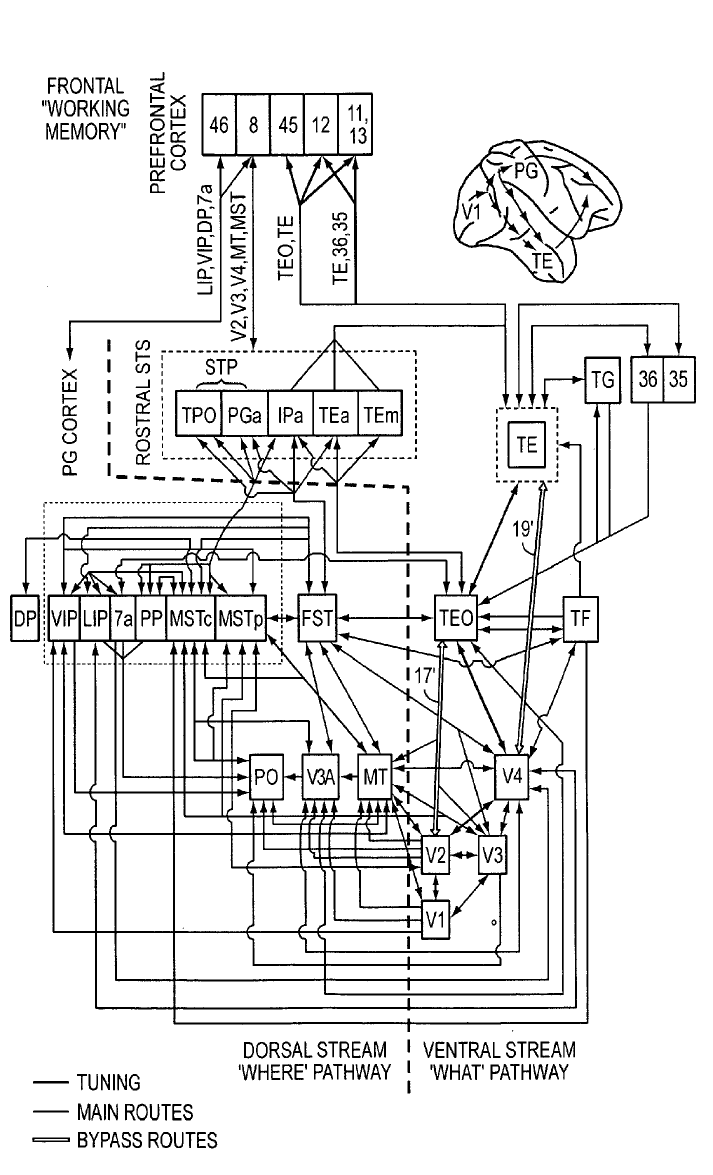
\includegraphics[width=0.82\textwidth]{images/patent_model.png}
	\caption{Model przedstawiający połączenia między elementami kory wzrokowej człowieka oraz jego podział na dwa szlaki: brzuszny i grzbietowy, które ściśle ze sobą są powiązane \cite{USPatent}.}
	\label{fig:USPatent_model}
\end{figure}

\begin{figure}[ht]
	\centering
	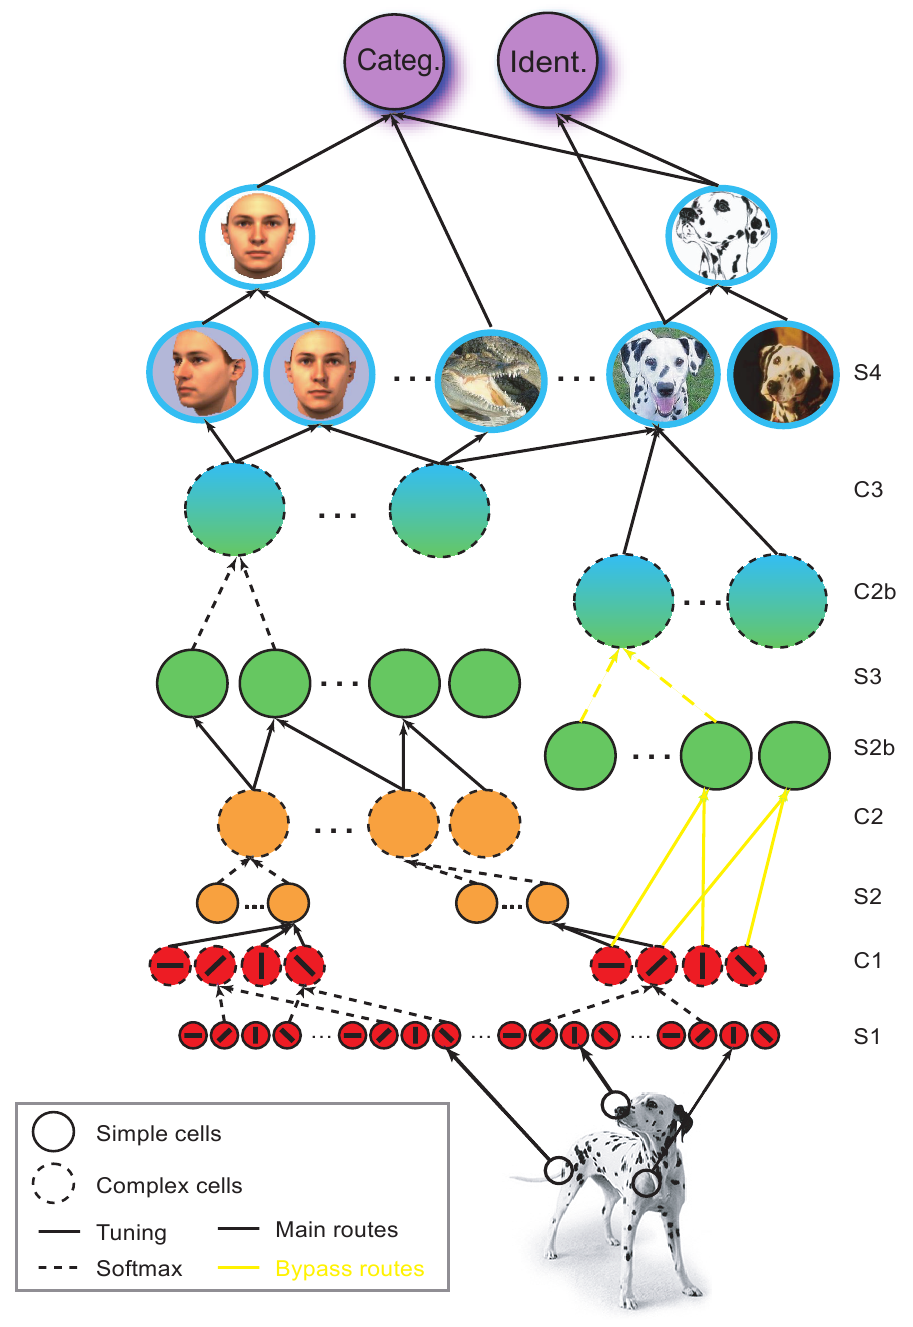
\includegraphics[width=0.9\textwidth]{images/Poggio_book_struct.png}
	\caption{Struktura odzwierciedlająca hierarchię połączeń w modelu rozpoznawania obrazów \cite{Serre2005}.}
	\label{fig:Poggio_BookModel}
\end{figure}

\begin{figure}[ht]
	\centering
	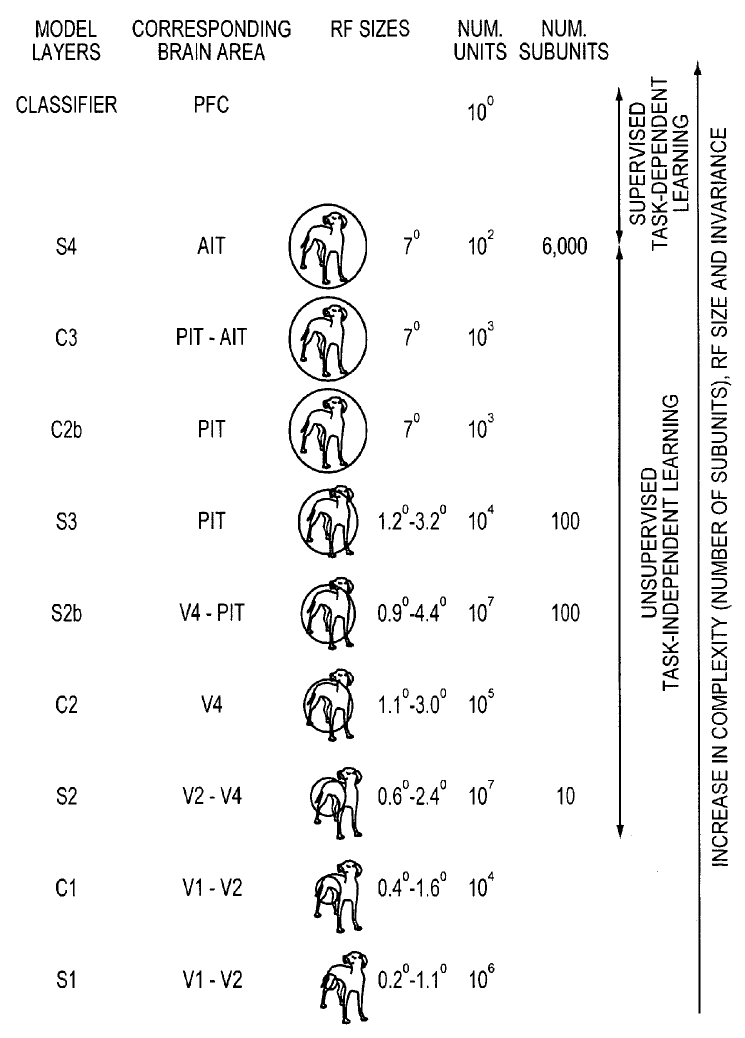
\includegraphics[width=0.91\textwidth]{images/patent_model_scale.png}
	\caption{Odzwierciedlenie zakresu szczegółowości na kolejnych poziomach modelu przedstawionego na rysunku \ref{fig:Poggio_BookModel} \cite{USPatent}.}
	\label{fig:USPatent_fineLevel}
\end{figure}

Sens takich połączeń, hierarchi można w bardzo prosty sposób wyjaśnić mając na uwadze to co się dzieje w ludzkim mózgu. Już na poziomie pierwszorzędowej kory wzrokowej, z informacji pobranych z ciała kolankowatego bocznego pobierane, tworzone są niewielkie krawędzie. Następnie -- wyżej się będzie poruszać w hierarchii, z tym większymi obiektami ma się do czynienia. Niewielkie krawędzie łączą się bowiem w większe, a następnie w złożone cechy, reprezentujące grupy krawędzi, nie będące współliniowymi. Opisywane poziomy szczegółowości dobrze przedstawione są na rysunku \ref{fig:USPatent_fineLevel} i należałoby patrzeć równocześnie na rysunek \ref{fig:Poggio_BookModel}, na którym każdy z poziomów szczegółowości jest umieszczony w hierarchii. Wyraźnie widać również, że poziom \texttt{S4} jest ostatnim w którym występuje tak zwane nienadzorowane uczenie, a wyższe warstwy są już klasyfikatorami, przypisującymi konkretnym obiektom konkretne klasy. Co warto zauważyć, to fakt istnienia połączeń międzywarstwowych, który mimo, że po raz kolejny dobrze odzwierciedla połączenia w korze wzrokowej, komplikuje interpretację działania samego modelu.\\

\begin{figure}[ht]
	\centering
	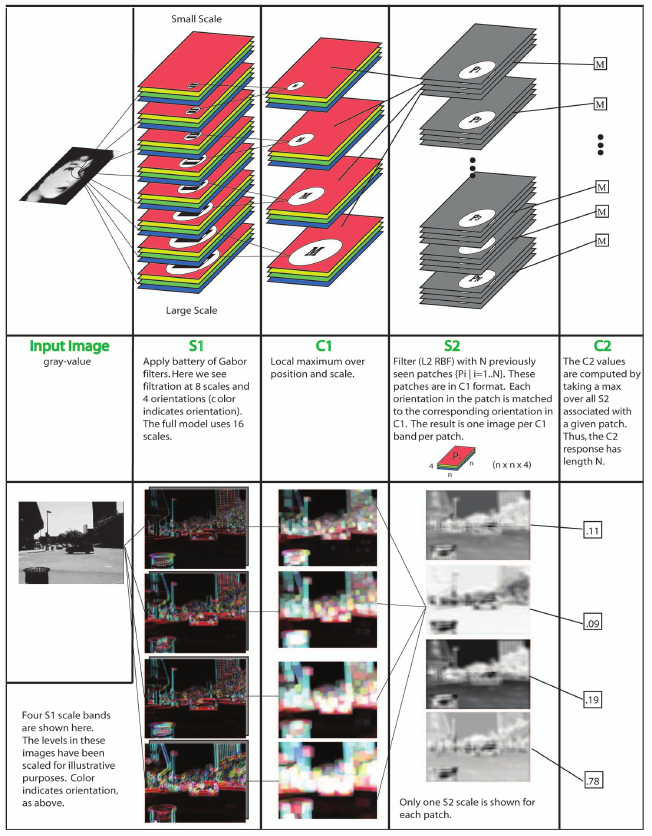
\includegraphics[width=\textwidth]{images/Poggio_model_implementation.png}
	\caption{Przedstawienie szczegółów dotyczących podstawowych bloków, z których jest złożony model z rysunku \ref{fig:Poggio_BookModel} \cite{Serre2007}.}
	\label{fig:HMax_model}
\end{figure}

Wchodząc natomiast w kwestie implementacyjne, czyli dotyczące realizacji modelu z rysunku \ref{fig:Poggio_BookModel} autorzy wniosku patentowego przedstawiają odpowiadające pierwszym czterem poziomom w hierarchii przekształcenia. Ich dokładny opis przedstawiony jest na rysunku \ref{fig:HMax_model}. W literaturze nazywa się ten model słowem \textit{HMAX}, które jak można przypuszczać wywodzi się od połączenia Hierarchiczności z operacją MAXimum, która jest jednym z najważniejszych przekształceń zachodzącym w modelu.\\

Przedstawiony etap \texttt{S1} na rysunku \ref{fig:HMax_model} stosuje opisane w załączniku \ref{aGabor} stosowanie filtru Gabora. Autorzy za istotne uznali nie tylko kąty, pod którymi funkcja Gabora jest w oknie zorientowana, ale i wielkość samego okna filtru. Co można przeczytać na opisywanym rysunku zdecydowali oni, że dużo istotniejsza jest skala od orientacji, przez co orientacje są tylko 4, natomiast skal 16. Każda orientacja na rysunku \ref{fig:HMax_model} oznaczona jest innym kolorem, a każde występujące pod sobą 4 różne kolory odpowiadają jednej skali -- wielkości okna filtru Gabora.\\

W etapie \texttt{C1} spośród otrzymanych wyników filtrowania jest wyciągane maximum ze względu na pozycję i skalę. W tej części wynikiem operacji maximum jest część przefiltrowanego obrazu, która wykazała się największą odpowiedzią spośród tych z sąsiedniej skali i orientacji.\\

Etap \texttt{S2} przedstawia ocenę wszystkich otrzymanych w poprzednim etapie elementów obrazu w stosunku do zapamiętanych przez model prototypów -- którymi są pewne elementy opisujące krawędzie (przypis autora). Ocena przebiega poprzez policzenie odległości euklidesowej między elementem zapamiętanym w modelu, a fragmentem obrazu z poprzedniego etapu. Dodatkowo ocena ta jest argumentem pewnej funkcji Gauso-podobnej, aby dodatkowo zmniejszyć znaczenie fragmentów obrazu, którym dużo brakuje do danych elementów modelu.\\

Jak się można było spodziewać, etap \texttt{C2} będzie polegał na zastosowaniu funkcji maximum globalnie, po wszystkich wynikach poprzedniego etapu.\\

Mimo, że przedstawiona -- jedna z wielu istniejących -- implementacja kończy przetwarzanie informacji wizualnych na poziomie \texttt{S2}, to można sobie wyobrazić kontynuację tego procesu, w którym na kolejnych poziomach są budowane coraz to bardziej złożone cechy. Na samym szczycie następuje natomiast klasyfikacja i przypisywanie otrzymanego w ten sposób wyniku do konkretnej klasy.

\subsection{Rozpoznawanie obiektów wywodzące się z podziału na komponenty}
\label{componentBasedObjectRecognition}
 
Co jest podkreślane bardzo często w świecie publikacji, przedstawiony model jest ciężki obliczeniowo i istnieje bardzo wiele jego modyfikacji, które nastawione są bardzo często na zwiększenie jego wydajności. Podobnie planował to zrobić autor wymienianej na początku tej części pracy magisterskiej \cite{Lopez2008}.\\


